% ----------------------------------------------------------------
%       Speech Signal Processing Toolkit (SPTK): version 3.0
%                      SPTK Working Group
% 
%                Department of Computer Science
%                Nagoya Institute of Technology
%                             and
%   Interdisciplinary Graduate School of Science and Engineering
%                Tokyo Institute of Technology
%                   Copyright (c) 1984-2000
%                     All Rights Reserved.
% 
% Permission is hereby granted, free of charge, to use and
% distribute this software and its documentation without
% restriction, including without limitation the rights to use,
% copy, modify, merge, publish, distribute, sublicense, and/or
% sell copies of this work, and to permit persons to whom this
% work is furnished to do so, subject to the following conditions:
% 
%   1. The code must retain the above copyright notice, this list
%      of conditions and the following disclaimer.
% 
%   2. Any modifications must be clearly marked as such.
%                                                                        
% NAGOYA INSTITUTE OF TECHNOLOGY, TOKYO INSITITUTE OF TECHNOLOGY,
% SPTK WORKING GROUP, AND THE CONTRIBUTORS TO THIS WORK DISCLAIM
% ALL WARRANTIES WITH REGARD TO THIS SOFTWARE, INCLUDING ALL
% IMPLIED WARRANTIES OF MERCHANTABILITY AND FITNESS, IN NO EVENT
% SHALL NAGOYA INSTITUTE OF TECHNOLOGY, TOKYO INSITITUTE OF
% TECHNOLOGY, SPTK WORKING GROUP, NOR THE CONTRIBUTORS BE LIABLE
% FOR ANY SPECIAL, INDIRECT OR CONSEQUENTIAL DAMAGES OR ANY
% DAMAGES WHATSOEVER RESULTING FROM LOSS OF USE, DATA OR PROFITS,
% WHETHER IN AN ACTION OF CONTRACT, NEGLIGENCE OR OTHER TORTIOUS
% ACTION, ARISING OUT OF OR IN CONNECTION WITH THE USE OR
% PERFORMANCE OF THIS SOFTWARE.
% ----------------------------------------------------------------
%
\name{df2}{second order dimension digital filter}{digital filter}

\begin{synopsis}
 \item[df2] [ --f $f_0$ ] [ --p $f_1 \; b_1$ ] [ --z $f_2 \; b_2$ ] 
	    [ {\em infile} ]
\end{synopsis}

\begin{qsection}{DESCRIPTION}
{\em df2} filters data from {\em infile} (or standard output) 
with a 2nd order digital filter, 
sending the result to standard output.
The central frequency and frequency band can
  be assigned through the options.
  The filter transfer function is
  \[
   H(z)=\frac{1-2\exp(-\pi b_2/f_0)\cos(2\pi f_2/f_0)z^{-1} +
	\exp(-2\pi b_2/f_0)z^{-2}}
   {1-2\exp(-\pi b_1/f_0)\cos(2\pi f_1/f_0)z^{-1}+\exp(-2\pi b_1/f_0)z^{-2}}
  \]
 If this command is used in cascade, an arbitrary filter can be
 designed using the options --p and --z.
 Input and output data are in float format.
\end{qsection}

\begin{options}
	\argm{f}{f_0}{sampling frequency $f_0$ [Hz]}{10000}
	\argm{p}{f_1 \; b_1}{center frequency $f_1$ [Hz]
                and band width $b_1$ [Hz] of pole}{N/A}
	\argm{z}{f_2 \; b_2}{center frequency $f_2$ [Hz]
                and band width $b_2$ [Hz] of zero}{N/A}
\end{options} 

\begin{qsection}{EXAMPLE}
The command below gives the impulse response of a filter with
a pole at 2000Hz and a frequency band of 200Hz:
\begin{quote}
 \verb!impulse | df2 -p 2000 200 !
\end{quote}
\hspace{3cm}
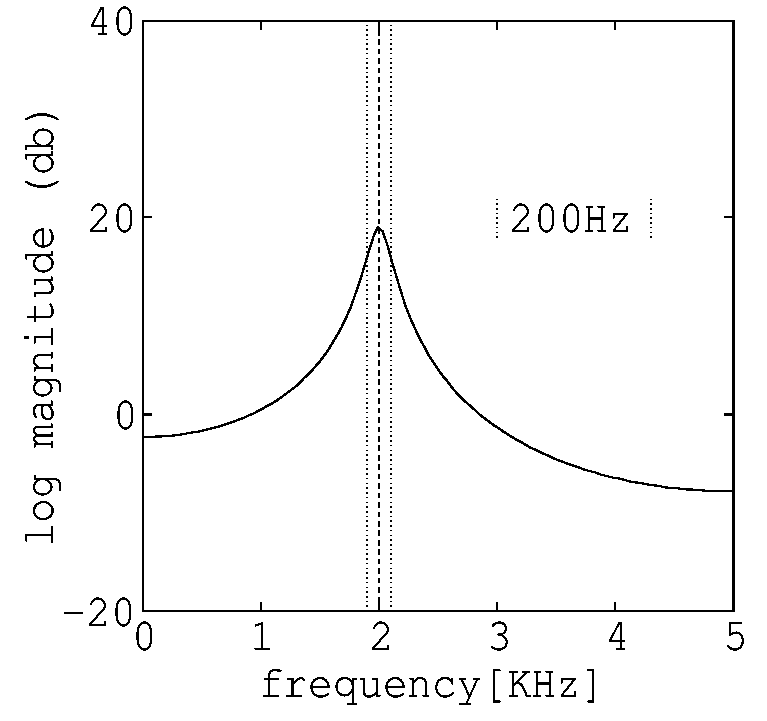
\includegraphics[width=4cm]{fig/df2.eps}
\end{qsection}
